\appendix

\chapter{Suivi de projet}

\begin{description}
\item[14 janvier~:] Premier contact avec l'équipe d'IBM, réunion de démarrage du projet au LINA\footnote{Laboratoire d'Informatique de Nantes-Atlantique} avec Mme~Martin, Mme~Amato et M.~Sunyé~; aperçu de la problématique et des besoins.
\item[19 janvier (matin)~:] Réunion hebdomadaire au LINA avec M.~Sunyé~; mise en place du dépôt Subversion.
\item[19 janvier (après-midi)~:] Premier contact avec M.~Brunat du Relai Handicap~; spécifications des besoins de l'utilisateur de l'outil, précisions sur les contraintes techniques.
\item[26 janvier~:] Réunion hebdomadaire~; discussion sur de nouveaux concepts à ajouter à l'outil.
\item[2 février~:] Réunion hebdomadaire~; répartition de tâches~: description des cas d'utilisation, spécification du schéma de la base de données embarquée, storyboard de l'IHM.
\item[9 février~:] Réunion au LINA avec l'équipe de Polytech'~; présentation des solutions architecturales envisageables, partage d'idées pour l'ergonomie de l'IHM.
\item[16 et 23 février~:] Réunions hebdomadaires~; discussion sur l'avancement du projet, engagement de démarche pour le choix du microphone.
\item[2 mars~:] Réunion hebdomadaire~; mise en place du système de gestion de projet Basecamp\footnote{Projet Basecamp -- \url{https://master-alma.basecamphq.com/}}
\item[9 mars~:] Réunion hebdomadaire~; découverte et exploitation du serveur d'intégration Hudson et du serveur de contrôle de qualité de code Sonar.
\item[11 mars~:] Conférence téléphonique au LINA avec M.~Sunyé, M.~Brunat et l'équipe d'IBM~; discussion sur l'avancement du projet et sur les difficultés rencontrées.
\item[16 mars~:] Dernière réunion hebdomadaire~; définition de nouvelles tâches à réaliser.
\item[25 mars~:] Soutenance du projet~; exposé et démonstration de l'outil.
\end{description}


\chapter{Diagramme de Gantt}

Bien que nous ne nous soyons pas vraiment attribués de fonctions telles que développeur, architecte ou même chef de projet, nous nous sommes répartis une grande partie des tâches à accomplir pour l'avancement du projet.
En conséquent, nous obtenons le diagramme de Gantt de la figure~\ref{fig:gantt}.

\begin{figure}[h!]
 \centering
 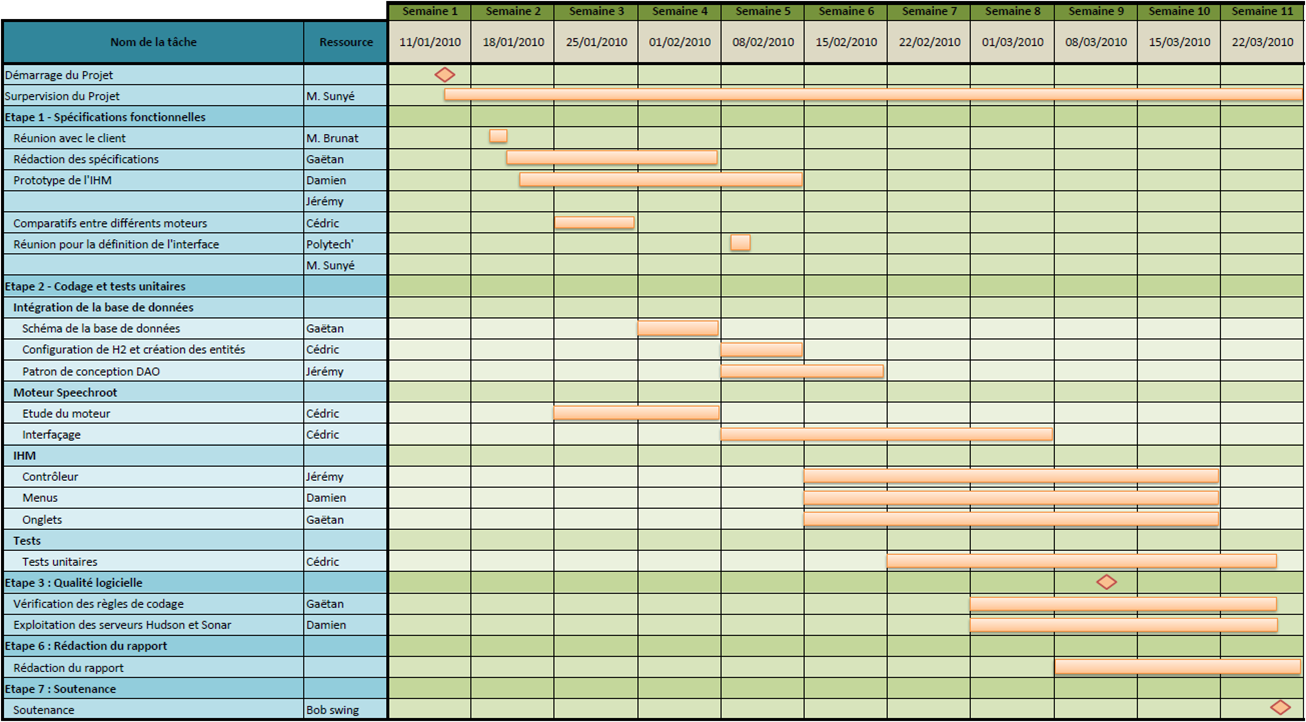
\includegraphics[width=16cm]{./images/Gantt.png}
 \caption{Diagramme de Gantt}
 \label{fig:gantt}
\end{figure}


\printindex
